\documentclass[aps,prd,twocolumn,superscriptaddress,nofootinbib,floatfix]{revtex4-2}

\usepackage[utf8]{inputenc}
\usepackage{amsmath,amssymb}
\usepackage{mathtools}
\usepackage{booktabs}
\usepackage{graphicx}
\usepackage{hyperref}
\usepackage{xcolor}
\usepackage{slashed}
\usepackage{amsthm}
\newtheorem{theorem}{Theorem}[section]
\newtheorem{proposition}[theorem]{Proposition}
\newtheorem{lemma}[theorem]{Lemma}
\newtheorem{corollary}[theorem]{Corollary}
\theoremstyle{definition}
\newtheorem{definition}[theorem]{Definition}
\theoremstyle{remark}
\newtheorem{remark}[theorem]{Remark}

\hypersetup{
  colorlinks=true,
  linkcolor=blue!60!black,
  citecolor=blue!60!black,
  urlcolor=blue!60!black,
  pdfauthor={David Alfyorov},
  pdftitle={Nonlocal one-loop form factors of the spectral action with Standard Model content},
  pdfsubject={doi:10.22541/au.177507193.33027854/v1}
}

%%% Custom commands
\newcommand{\Weylsq}{C_{\mu\nu\rho\sigma}C^{\mu\nu\rho\sigma}}
\newcommand{\Ricsq}{R_{\mu\nu}R^{\mu\nu}}
\newcommand{\Riemsq}{R_{\mu\nu\rho\sigma}R^{\mu\nu\rho\sigma}}
\newcommand{\dd}{\mathrm{d}}
\newcommand{\erfi}{\operatorname{erfi}}
\newcommand{\tr}{\operatorname{tr}}
\newcommand{\Tr}{\operatorname{Tr}}

\begin{document}

\title{Nonlocal one-loop form factors of the spectral action\\with Standard Model content}

\author{David Alfyorov}
\affiliation{Independent researcher}
\email{davidich.alfyorov@gmail.com}

\begin{abstract}
We compute the matter-induced nonlocal one-loop curvature-squared form factors
$F_1(\Box/\Lambda^2)$ and $F_2(\Box/\Lambda^2,\xi)$ relevant to the spectral
action $S = \Tr\,f(D^2/\Lambda^2)$, for Standard Model field content:
4 real scalars (Higgs doublet), $45/2$ Dirac-equivalent fermions
(3 generations), and 12 gauge bosons
($\mathrm{SU}(3)\times\mathrm{SU}(2)\times\mathrm{U}(1)$).
Using Barvinsky--Vilkovisky covariant perturbation
theory~\cite{Barvinsky:1985an,Barvinsky:1987uw} and the Codello--Zanusso
nonlocal heat kernel~\cite{Codello:2012kq}, we derive closed-form reduced
kernels $h_C^{(s)}(x)$ and $h_R^{(s)}(x)$ for each spin sector
($s = 0, 1/2, 1$) in the Weyl basis $\{C^2, R^2\}$, with step-by-step
assembly from the five universal CZ structure functions. For spin-1, we provide
the complete Faddeev--Popov ghost derivation with two minimally coupled scalar
ghosts. The Standard Model assembly yields
$\alpha_C = 13/120$ (Weyl-squared, $\xi$-independent) and
$\alpha_R(\xi) = 2(\xi - 1/6)^2$ ($R^2$, Higgs non-minimal coupling only),
reproducing all known local
limits~\cite{Gilkey:1975iq,Vassilevich:2003xt,Codello:2008vh,Stelle:1976gc}.
After removing apparent singularities at $z = 0$, the reduced form factors
are proven to be entire functions of $z = \Box/\Lambda^2$ of order~1 and
type~$1/4$; consequently, the form factors themselves introduce no propagator
poles. Ghost poles arise from zeros of the dressed propagator, which we derive
from the full linearized quadratic action using Barnes--Rivers spin
projectors~\cite{Barnes:1965,Rivers:1964}. This yields effective masses
$m_2 = \Lambda\sqrt{60/13}$ (spin-2) and
$m_0 = \Lambda/\sqrt{6(\xi - 1/6)^2}$ (spin-0), with the scalar mode
decoupling at conformal coupling $\xi = 1/6$.
All results are independently verified by triple computer algebra
(SymPy, cadabra2~\cite{Peeters:2007wn}, FORM~\cite{Vermaseren:2000nd}),
arbitrary-precision numerical evaluation ($\geq 100$ digits), and Lean~4
formal proofs for the coefficient arithmetic.
\end{abstract}

\pacs{04.62.+v, 04.60.-m, 11.10.Jj, 04.50.Kd}
\keywords{spectral action, heat kernel, form factors, quadratic gravity,
Standard Model, noncommutative geometry}

\maketitle

% ============================================================
\section{Introduction}
\label{sec:intro}
% ============================================================

The spectral action principle~\cite{Connes:1994yd,Chamseddine:1996zu,Chamseddine:2006ep}
provides a geometric origin for both gravitational and gauge interactions:
the bosonic action is given by $S = \Tr\,f(D^2/\Lambda^2)$, where $D$ is the
Dirac operator of a noncommutative geometry, $\Lambda$ is a cutoff scale, and
$f$ is a positive even function. At the classical level, the heat kernel
expansion of this trace reproduces the Einstein--Hilbert action, cosmological
constant, and Yang--Mills terms from the first few Seeley--DeWitt
coefficients~\cite{Chamseddine:2010ud,vanSuijlekom:2014pya}.

Beyond the leading Seeley--DeWitt approximation, the spectral action generates
\emph{nonlocal} curvature-squared terms characterized by momentum-dependent
form factors $F_1(\Box/\Lambda^2)$ and $F_2(\Box/\Lambda^2,\xi)$. These form
factors encode the \emph{matter-induced} contribution to the one-loop
curvature-squared effective action at $\mathcal{O}(\mathcal{R}^2)$: they arise
from functional traces over matter fields (scalars, fermions, gauge bosons)
propagating on a fixed curved gravitational background. The graviton
self-energy contributions, which would constitute the full quantum gravitational
effective action, are not computed here; they require a separate treatment of
the metric fluctuation operator, its gauge-fixing, and the gravitational ghost
sector~\cite{Stelle:1976gc,Buchbinder:1992rb}. Nevertheless, the matter-induced
form factors already determine the modified graviton propagator structure,
effective masses, and the UV behavior when matter-loop contributions dominate.

The Barvinsky--Vilkovisky (BV) covariant perturbation
theory~\cite{Barvinsky:1985an,Barvinsky:1987uw,Barvinsky:1990up,Barvinsky:2009gw} provides the
general framework for computing such form factors for any generalized Laplacian
$\Delta = -(g^{\mu\nu}\nabla_\mu\nabla_\nu + E)$ on a vector bundle over a
curved manifold. The Codello--Zanusso (CZ) diagrammatic heat kernel
technique~\cite{Codello:2012kq} gives explicit expressions for the five
independent structure functions
($f_{\text{Ric}}, f_R, f_{RU}, f_U, f_\Omega$) in terms of a universal
master function $\varphi(x)$, which depends only on the proper-time parameter
and is independent of the profile function $f$ at
$\mathcal{O}(\mathcal{R}^2)$ (see Appendix~\ref{app:profile} for a proof).
The Seeley--DeWitt coefficients and their role in spectral geometry are
reviewed
in~\cite{DeWitt:1964mxt,Gilkey:1975iq,Vassilevich:2003xt,Avramidi:2000bm,Fursaev:2011zz}.

The per-spin form factors for individual Laplace-type operators were obtained
by BV~\cite{Barvinsky:1987uw,Barvinsky:1990up} and
CZ~\cite{Codello:2012kq}; local limits ($\beta$-function coefficients) were
tabulated for matter fields by CPR~\cite{Codello:2008vh} and in the textbook
by Parker and Toms~\cite{Parker:2009uva}. One-loop corrections to the
spectral action were studied by van Nuland and van
Suijlekom~\cite{vanNuland:2022xkm}, and the spectral-action framework for
higher-derivative gravity was analyzed by Mistry, Pinzul, and
Rachwa{\l}~\cite{Mistry:2020xqh}. The present contribution assembles the
full Standard Model (SM) per-spin form factors into SM-specific quantities
($\alpha_C$, $\alpha_R(\xi)$, $c_1/c_2$) that have not been previously
reported, proves the entire-function property of the SM totals, and derives
the dressed graviton propagator from the complete linearized quadratic action.

The SM particle content consists of 4 real scalars (Higgs doublet),
$N_f = 45$ Weyl fermions (equivalently $N_D = 45/2$ Dirac fermions in 3
generations), and 12 gauge bosons of $\mathrm{SU}(3) \times \mathrm{SU}(2)
\times \mathrm{U}(1)$. The counting convention follows
CPR~\cite{Codello:2008vh}.

The main results are:
\begin{itemize}
\item Closed-form expressions for the reduced form factors
  $h_C^{(s)}(x)$ and $h_R^{(s)}(x)$ for $s = 0, 1/2, 1$ in the Weyl basis
  $\{C^2, R^2\}$, with complete step-by-step derivation of the BV/CZ assembly
  for each spin sector (Secs.~\ref{sec:scalar}--\ref{sec:vector}).
\item The SM totals $\alpha_C = 13/120$ ($\xi$-independent, determined by SM
  content) and $\alpha_R(\xi) = 2(\xi - 1/6)^2$ (depending only on the Higgs
  non-minimal coupling $\xi$), with the local $R^2$ coefficient vanishing at
  conformal coupling $\xi = 1/6$ (Sec.~\ref{sec:sm}).
\item A proof that the reduced form factors, after removal of apparent
  singularities at $z = 0$, are entire functions of order~1 and type~$1/4$
  (Theorem~\ref{thm:entire}). As a consequence, the form factors introduce no
  propagator poles; ghost poles arise solely from zeros of the dressed
  propagator (Sec.~\ref{sec:entire}).
\item The dressed spin-2 and spin-0 propagators
  $\Pi_{TT}(z)$, $\Pi_s(z,\xi)$, derived from the full linearized quadratic
  action via Barnes--Rivers projectors, yielding effective masses
  $m_2 = \Lambda\sqrt{60/13}$, $m_0 = \Lambda/\sqrt{6(\xi - 1/6)^2}$ and the
  modified Newtonian potential (Sec.~\ref{sec:propagator}).
\item A systematic comparison with BV, CZ, CPR, Parker--Toms, Stelle, and the
  Donoghue effective field theory~\cite{Donoghue:1994dn,BjerrumBohr:2002kt}
  (Sec.~\ref{sec:comparison}).
\end{itemize}

The structure of the paper is as follows. Section~\ref{sec:setup} establishes
the conventions and reviews the BV/CZ formalism, including the
$f$-independence of the form factors at $\mathcal{O}(\mathcal{R}^2)$.
Sections~\ref{sec:scalar}--\ref{sec:vector} derive the form factors for each
spin sector with explicit BV assembly.
Section~\ref{sec:sm} assembles the SM totals.
Section~\ref{sec:entire} proves the entire-function property.
Section~\ref{sec:propagator} derives the dressed propagator and effective
masses. Section~\ref{sec:uv} discusses UV asymptotics.
Section~\ref{sec:comparison} compares with existing results, including the
Donoghue EFT. Section~\ref{sec:discussion} discusses implications for
asymptotic safety and nonlocal gravity. We conclude in
Sec.~\ref{sec:conclusions}.

Throughout this paper we use the Euclidean signature $(+,+,+,+)$, natural
units $c = \hbar = 1$, and the generalized Laplacian convention
$\Delta = -(g^{\mu\nu}\nabla_\mu\nabla_\nu + E)$ of Barvinsky and
Vilkovisky~\cite{Barvinsky:1985an}. The CZ endomorphism is
$\mathbf{U} = -E$. The Lorentzian continuation to $(-,+,+,+)$ signature is
discussed in Sec.~\ref{sec:discussion}. Convention tables are collected in
Appendix~\ref{app:conventions}. A summary of the principal results is given
in Table~\ref{tab:summary}.


% ============================================================
\section{Setup and Conventions}
\label{sec:setup}
% ============================================================

\subsection{Generalized Laplacian and spectral action}

We consider a closed (compact, boundaryless) Riemannian spin 4-manifold
$(M,g)$. For each matter field of spin $s$, the one-loop effective action is
\begin{equation}
  \Gamma^{(s)} = \frac{(-1)^{2s}}{2}\,\Tr\ln\Delta^{(s)}\,,
  \label{eq:one-loop}
\end{equation}
where $\Delta^{(s)}$ is the generalized Laplacian of the corresponding
kinetic operator, and $(-1)^{2s} = +1$ for bosons, $-1$ for fermions. At
$\mathcal{O}(\mathcal{R}^2)$, the curvature-squared sector of the effective
action takes the form
\begin{equation}
  \Gamma\Big|_{\mathcal{R}^2}
  = \int_M \dd^4x\,\sqrt{g}\,\bigl[
    F_1(z)\,\Weylsq + F_2(z,\xi)\,R^2
  \bigr]\,,
  \label{eq:spectral-action}
\end{equation}
where $z \equiv \Box/\Lambda^2$ and $\Lambda$ is the spectral cutoff scale.
The form factors $F_i$ are the central objects of this paper.

For a generalized Laplacian $\Delta = -(g^{\mu\nu}\nabla_\mu\nabla_\nu + E)$
acting on a vector bundle of rank $d_V$ (so that $\tr\,\mathbf{1} = d_V$),
the CZ endomorphism is $\mathbf{U} = -E$ and the bundle curvature is
$\Omega_{\mu\nu} = [\nabla_\mu, \nabla_\nu]$ acting on sections of the
bundle. We write
\begin{equation}
  F_i^{(s)}(z) = \frac{h_i^{(s)}(z)}{16\pi^2}\,,\quad i = C, R\,,
  \label{eq:Fi-hi-def}
\end{equation}
where $h_C^{(s)}$ and $h_R^{(s)}$ are the \emph{reduced} form factors.
Their local limits $\beta_W^{(s)} \equiv h_C^{(s)}(0)$ and
$\beta_R^{(s)} \equiv h_R^{(s)}(0)$ are the one-loop $\beta$-function
coefficients of the $C^2$ and $R^2$ operators. In our convention, the fermionic sign from~\eqref{eq:one-loop} is not
applied as an explicit overall factor; it is encoded in the assembly rules
through the operator data (Sec.~\ref{sec:assembly}). For the SM spins
$s = 0, 1/2, 1$, the resulting $h_C^{(s)}(0)$ is positive for bosons and
negative for the Dirac fermion, but this pattern does not extend to all
spins (see Sec.~\ref{sec:rs}).

\subsection{From heat-kernel kernels to spectral-action form factors}
\label{sec:smearing}

The spectral action $S = \Tr\,f(D^2/\Lambda^2)$ depends on a profile
function~$f$. We now make precise how the form factors depend on~$f$, and
under what conditions they are $f$-independent.

If $f$ admits a Laplace representation
$f(u) = \int_0^\infty \dd\alpha\,\tilde{f}(\alpha)\,e^{-\alpha u}$,
then the spectral action at $\mathcal{O}(\mathcal{R}^2)$ becomes
\begin{equation}
  S_f\big|_{\mathcal{R}^2}
  = \frac{1}{16\pi^2}\int_M \dd^4x\,\sqrt{g}\,\bigl[
    \mathcal{H}_C(z;f)\,\Weylsq + \mathcal{H}_R(z,\xi;f)\,R^2
  \bigr]\,,
  \label{eq:smeared-action}
\end{equation}
where the \emph{profile-smeared} form factors are
\begin{equation}
  \mathcal{H}_i(z;f) = \int_0^\infty \dd\alpha\,\tilde{f}(\alpha)\,
    h_i(\alpha z)\,,\quad i = C,R\,.
  \label{eq:smearing}
\end{equation}
Here $h_i$ denotes the \emph{reduced kernel} corresponding to the exponential
profile $f(u) = e^{-u}$ (i.e.,
$\tilde{f}(\alpha) = \delta(\alpha - 1)$). The reduced kernels, built from
the master function $\varphi(x)$, are universal --- they depend only on the
Laplace-type operator and not on the spectral profile. The
profile dependence enters solely through the smearing~\eqref{eq:smearing}.

\begin{remark}
All explicit closed formulas in this paper are reduced kernels $h_i$. They
coincide with the spectral-action form factors only for the exponential
profile, or more generally for any delta-supported proper-time measure.
\end{remark}

A direct consequence of~\eqref{eq:smearing} is the profile dependence of the
local coefficients:
\begin{equation}
  \mathcal{H}_i(0;f) = h_i(0)\,f(0)\,,
  \label{eq:f0-factor}
\end{equation}
since $\int_0^\infty \tilde{f}(\alpha)\,\dd\alpha = f(0)$.
Hence the \emph{ratios} of local curvature-squared couplings (e.g.\
$c_1/c_2$) are profile-independent, while the overall normalization is
proportional to $f(0)$. For the SM local coefficients:
\begin{equation}
  \alpha_C^{\text{loc}} = \frac{13}{120}\,f(0)\,,\qquad
  \alpha_R^{\text{loc}} = 2\,f(0)\!\left(\xi - \frac{1}{6}\right)^{\!2}\,.
  \label{eq:alphaC-local-f}
\end{equation}
Throughout this paper, we set $f(0) = 1$ (exponential profile) unless
otherwise stated.

\subsection{Master function}

All form factors are built from the universal master function
\begin{equation}
  \varphi(x) = \int_0^1 \dd\alpha\, e^{-\alpha(1-\alpha)x}\,,
  \label{eq:phi-def}
\end{equation}
with the closed form
\begin{equation}
  \varphi(x) = e^{-x/4}\sqrt{\frac{\pi}{x}}\;\erfi\!\left(\frac{\sqrt{x}}{2}\right)\,.
  \label{eq:phi-closed}
\end{equation}
Key properties:
$\varphi(0) = 1$,
$\varphi'(0) = -1/6$,
and Taylor coefficients $a_n = (-1)^n\,n!/(2n+1)!$, so that
$\varphi(x) = \sum_{n=0}^\infty a_n\,x^n$ with infinite radius of
convergence (the ratio test gives $|a_{n+1}/a_n| \to 0$). In particular,
$\varphi$ is an entire function of order~1 and type~$1/4$
(Fig.~\ref{fig:phi}). The large-$x$ asymptotic expansion is
\begin{equation}
  \varphi(x) = \frac{2}{x} + \frac{4}{x^2} + \frac{24}{x^3}
    + \frac{240}{x^4} + \mathcal{O}(x^{-5})\,,
  \label{eq:phi-uv}
\end{equation}
which is an asymptotic (divergent) series, Borel-summable to the exact
$\varphi$.

\begin{figure}[t]
  \centering
  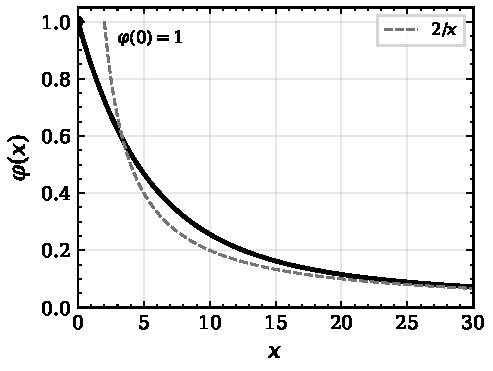
\includegraphics[width=\columnwidth]{figures/fig_phi.pdf}
  \caption{The master function $\varphi(x)$, where
  $x = \Box/\Lambda^2$. Starting from $\varphi(0) = 1$, the function
  decays monotonically and approaches the asymptotic form $2/x$
  (dashed) for $x \gg 1$.}
  \label{fig:phi}
\end{figure}

\subsection{CZ structure functions}

The five CZ structure functions~\cite{Codello:2012kq} are:
\begin{subequations}
\label{eq:CZ-ff}
\begin{align}
  f_{\text{Ric}}(x) &= \frac{1}{6x} + \frac{\varphi - 1}{x^2}\,,
  \label{eq:fRic}\\
  f_R(x) &= \frac{\varphi}{32} + \frac{\varphi}{8x}
    - \frac{7}{48x} - \frac{\varphi - 1}{8x^2}\,,
  \label{eq:fR}\\
  f_{RU}(x) &= -\frac{\varphi}{4} - \frac{\varphi - 1}{2x}\,,
  \label{eq:fRU}\\
  f_U(x) &= \frac{\varphi}{2}\,,
  \label{eq:fU}\\
  f_\Omega(x) &= -\frac{\varphi - 1}{2x}\,.
  \label{eq:fOmega}
\end{align}
\end{subequations}
Their local limits are $f_{\text{Ric}}(0) = 1/60$, $f_R(0) = 1/120$,
$f_{RU}(0) = -1/6$, $f_U(0) = 1/2$, $f_\Omega(0) = 1/12$.

\subsection{Weyl basis assembly}
\label{sec:assembly}

The BV/CZ expansion of the $\mathcal{O}(\mathcal{R}^2)$ heat kernel trace
for a single field with operator data
$(d_V, \mathbf{U}, \Omega_{\mu\nu})$ contains five universal structure
functions~\cite{Barvinsky:1987uw,Codello:2012kq}. After the proper-time
integration, the reduced kernels $h_C, h_R$ are assembled from:
\begin{align}
  \frac{1}{16\pi^2}\bigl[h_C\,\Weylsq &+ h_R\,R^2\bigr]
  \longleftarrow
  d_V\,f_{\text{Ric}}\,\Ricsq
  + d_V\,f_R\,R^2  \nonumber\\
  &+ R\,f_{RU}\,\tr(\mathbf{U})
  + \tr(\mathbf{U}\,f_U\,\mathbf{U})  \nonumber\\
  &+ \tr(\Omega_{\mu\nu}\,f_\Omega\,\Omega^{\mu\nu})\,,
  \label{eq:CZ-expansion}
\end{align}
where the conversion from the right-hand side (CZ basis) to the left-hand
side (Weyl basis) uses~\eqref{eq:GB-conversion}. The statistics sign
$(-1)^{2s}$ is \emph{not} applied as an extra overall factor; it is
already encoded in the operator data (specifically, in the sign and magnitude
of $\tr(\Omega^2)$ and $\mathbf{U}$) for each spin sector.
The five CZ functions act on the \emph{spacetime} argument
$x = \Box/\Lambda^2$, while the traces are over \emph{bundle} indices only.
The assembly into the Weyl basis $\{C^2, R^2\}$ proceeds by converting the
curvature invariants using the Gauss--Bonnet identity in $d = 4$ (modulo the
topological Euler density
$E_4 = \Riemsq - 4\Ricsq + R^2$):
\begin{subequations}
\label{eq:GB-conversion}
\begin{align}
  \Ricsq &= \tfrac{1}{2}\Weylsq + \tfrac{1}{3}R^2\,,
  \label{eq:GB-Ric}\\
  \Riemsq &= 2\,\Weylsq + \tfrac{1}{3}R^2\,.
  \label{eq:GB-Riem}
\end{align}
\end{subequations}

The key step, which differs between spin sectors, is the evaluation of
$\tr(\mathbf{U}\,f_U\,\mathbf{U})$ and
$\tr(\Omega\,f_\Omega\,\Omega)$:
\begin{itemize}
\item If $\mathbf{U} \propto R\cdot\mathbf{1}$ (scalar or proportional to
  the identity, as for spin-0 and spin-1/2), then
  $\tr(\mathbf{U}\,f_U\,\mathbf{U}) \propto R^2 \cdot f_U$, contributing
  only to the $R^2$ channel.
\item If $\mathbf{U}$ is matrix-valued (e.g., $U^\mu{}_\nu = R^\mu{}_\nu$
  for spin-1), then
  $\tr(\mathbf{U}\,f_U\,\mathbf{U}) = f_U\,\Ricsq$, which contributes to
  \emph{both} $C^2$ and $R^2$ via~\eqref{eq:GB-Ric}.
\end{itemize}
This distinction is the source of the nontrivial assembly structure for
higher spins and will be exhibited explicitly in
Secs.~\ref{sec:scalar}--\ref{sec:vector}.


% ============================================================
\section{Spin-0: Real Scalar}
\label{sec:scalar}
% ============================================================

\subsection{Operator data}

For a real scalar field with non-minimal coupling $\xi R\phi^2/2$, the
generalized Laplacian is
$\Delta^{(0)} = -\Box + \xi R$ (i.e., $E = -\xi R$ in the BV convention
$\Delta = -(\Box + E)$), giving operator data:
\begin{equation}
  d_V = 1\,,\quad \mathbf{U} = \xi R\,,\quad
  \Omega_{\mu\nu} = 0\,.
  \label{eq:scalar-data}
\end{equation}
The endomorphism $\mathbf{U} = \xi R$ is scalar-valued (proportional to the
identity on the trivial bundle), and the bundle curvature vanishes since
the scalar field carries no internal indices.

\subsection{BV/CZ assembly}

The five terms in~\eqref{eq:CZ-expansion} give:
\begin{center}
\renewcommand{\arraystretch}{1.15}
\begin{tabular}{@{}llc@{}}
  \toprule
  Term & Curvature structure & Invariant \\
  \midrule
  $d_V\,f_{\text{Ric}}\,\Ricsq$ & $1 \cdot f_{\text{Ric}} \cdot \Ricsq$ &
    $\Ricsq$ \\
  $d_V\,f_R\,R^2$ & $1 \cdot f_R \cdot R^2$ & $R^2$ \\
  $R\,f_{RU}\,\tr(\mathbf{U})$ & $\xi\,f_{RU}\,R^2$ & $R^2$ \\
  $\tr(\mathbf{U}\,f_U\,\mathbf{U})$ & $\xi^2\,f_U\,R^2$ & $R^2$ \\
  $\tr(\Omega\,f_\Omega\,\Omega)$ & $0$ & --- \\
  \bottomrule
\end{tabular}
\end{center}
Since $\mathbf{U} = \xi R$ is scalar-valued,
$\tr(\mathbf{U}\,f_U\,\mathbf{U}) = \xi^2 R^2\,f_U$ contributes only to
$R^2$, not to $C^2$.

Converting $\Ricsq$ to the Weyl basis via~\eqref{eq:GB-Ric}:
\begin{subequations}
\label{eq:scalar-ff}
\begin{align}
  h_C^{(0)}(x) &= \tfrac{1}{2}\,f_{\text{Ric}}(x)
    = \frac{1}{12x} + \frac{\varphi - 1}{2x^2}\,,
  \label{eq:hC0}\\
  h_R^{(0)}(x,\xi) &= \tfrac{1}{3}f_{\text{Ric}}(x) + f_R(x)
    + \xi\,f_{RU}(x) + \xi^2\,f_U(x)\,.
  \label{eq:hR0}
\end{align}
\end{subequations}

\begin{lemma}[$\xi$-independence of $h_C^{(0)}$]
\label{lem:xi-indep}
The Weyl coefficient $h_C^{(0)}$ is independent of $\xi$. This holds because
$\mathbf{U} = \xi R$ is proportional to the scalar curvature, which is the
trace of the Ricci tensor: $R = g^{\mu\nu}R_{\mu\nu}$. The Weyl tensor is
traceless ($g^{\mu\nu}C_{\mu\alpha\nu\beta} = 0$), so only $\Ricsq$ appears
in the $C^2$ channel, and $\Ricsq$ comes solely from Term~1 (the
$f_{\text{Ric}}$ term), which is $\xi$-independent.
\end{lemma}

\subsection{Pole removability}

\begin{lemma}[Removability of $h_C^{(0)}$ at $x = 0$]
\label{lem:pole-scalar}
The apparent pole of $h_C^{(0)}(x) = 1/(12x) + (\varphi - 1)/(2x^2)$ at
$x = 0$ is removable. \emph{Proof.} Using the shifted-index formula
$h_C^{(0)}(x) = \sum_{n \geq 0}\tfrac{1}{2}a_{n+2}\,x^n$ with
$a_n = (-1)^n n!/(2n+1)!$, the poles are manifestly absent. The leading
term is $\tfrac{1}{2}a_2 = 1/120$, confirming analyticity at $x = 0$.
The Taylor expansion is
$h_C^{(0)}(x) = 1/120 - x/1680 + \mathcal{O}(x^2)$.
\end{lemma}

\subsection{Local limits}

\begin{equation}
  \beta_W^{(0)} = h_C^{(0)}(0) = \frac{1}{120}\,,\qquad
  \beta_R^{(0)}(\xi) = h_R^{(0)}(0,\xi)
    = \frac{1}{2}\!\left(\xi - \frac{1}{6}\right)^{\!2}\,.
  \label{eq:beta-scalar}
\end{equation}
The $R^2$ coefficient vanishes at conformal coupling $\xi = 1/6$, reflecting
the conformal invariance of the massless conformally-coupled scalar in
$d = 4$~\cite{Parker:2009uva}. For $\xi \neq 1/6$, the nonlocal form factor
$h_R^{(0)}(x, \xi)$ is nonzero for all $x > 0$. The individual form factors
are plotted in Figs.~\ref{fig:hC} and~\ref{fig:hR}.


% ============================================================
\section{Spin-1/2: Dirac Fermion}
\label{sec:dirac}
% ============================================================

\subsection{Operator data}

For a massless 4-component Dirac fermion, the Lichnerowicz formula gives the
squared Dirac operator:
\begin{equation}
  \slashed{D}^2 = -\bigl(\nabla^\mu\nabla_\mu - \tfrac{R}{4}\bigr)\,,
  \label{eq:lichnerowicz}
\end{equation}
which is a generalized Laplacian with $E = -R/4$ (note the sign:
$\Delta = -(\Box + E)$ in the BV convention), so that the CZ endomorphism is
\begin{equation}
  \mathbf{U} = -E = \frac{R}{4}\,\mathbf{1}_4\,.
  \label{eq:U-dirac}
\end{equation}
The spinor connection induces the bundle curvature
\begin{equation}
  (\Omega_{\mu\nu})^a{}_b = \frac{1}{4}\,R_{\mu\nu\rho\sigma}\,
    (\gamma^{\rho}\gamma^{\sigma})^a{}_b\,.
  \label{eq:Omega-dirac}
\end{equation}
The relevant traces are (using the $d = 4$ gamma-matrix identities
$\tr(\gamma^\mu\gamma^\nu) = 4\,g^{\mu\nu}$ and
$\tr(\gamma^{\mu\nu}\gamma^{\rho\sigma}) =
4(\delta^\mu_\rho\delta^\nu_\sigma - \delta^\mu_\sigma\delta^\nu_\rho)$):
\begin{subequations}
\label{eq:dirac-traces}
\begin{align}
  \tr(\mathbf{1}) &= 4\,,\\
  \tr(\mathbf{U}) &= R\,,\quad
  \tr(\mathbf{U}^2) = \frac{R^2}{4}\,,\\
  \tr(\Omega_{\mu\nu}\Omega^{\mu\nu})
    &= \frac{1}{16}\,R_{\mu\nu\rho\sigma}\,R^{\mu\nu\alpha\beta}\,
    \tr(\gamma^{\rho\sigma}\gamma_{\alpha\beta}) \nonumber\\
    &= -\frac{1}{2}\,\Riemsq\,.
  \label{eq:trOmega-dirac}
\end{align}
\end{subequations}
The sign in~\eqref{eq:trOmega-dirac} follows from the antisymmetry of
$R_{\mu\nu\rho\sigma}$ in the last pair and the trace identity
$\tr(\gamma^{\rho\sigma}\gamma_{\alpha\beta}) =
4(\delta^\rho_\alpha\delta^\sigma_\beta -
\delta^\rho_\beta\delta^\sigma_\alpha)$; contracting gives
$R_{\mu\nu\rho\sigma}R^{\mu\nu\rho\sigma} - R_{\mu\nu\rho\sigma}R^{\mu\nu\sigma\rho} = 2\,\Riemsq$,
then the factor $1/16 \times 4 \times 2 = 1/2$ with the relative minus from
the antisymmetry.

\subsection{BV/CZ assembly}

Since $\mathbf{U} = (R/4)\mathbf{1}_4$ is proportional to the identity,
$\tr(\mathbf{U}\,f_U\,\mathbf{U}) = (R^2/4)\,f_U$ contributes only to
$R^2$. The five terms in~\eqref{eq:CZ-expansion} give:
\begin{center}
\renewcommand{\arraystretch}{1.15}
\begin{tabular}{@{}lll@{}}
  \toprule
  Term & Contribution (unsigned) & Invariant \\
  \midrule
  Term~1 & $4\,f_{\text{Ric}}\,\Ricsq$ & $\Ricsq$ \\
  Term~2 & $4\,f_R\,R^2$ & $R^2$ \\
  Term~3 & $f_{RU}\,R^2$ & $R^2$ \\
  Term~4 & $\tfrac{1}{4}\,f_U\,R^2$ & $R^2$ \\
  Term~5 & $-\tfrac{1}{2}\,f_\Omega\,\Riemsq$ & $\Riemsq$ \\
  \bottomrule
\end{tabular}
\end{center}

Converting to the Weyl basis via~\eqref{eq:GB-conversion}:
\begin{subequations}
\label{eq:dirac-ff}
\begin{align}
  h_C^{(1/2)}(x) &= 2\,f_{\text{Ric}} - f_\Omega
  \label{eq:hC12-assembly}\\
  &= \frac{3\varphi - 1}{6x} + \frac{2(\varphi - 1)}{x^2}\,,
  \label{eq:hC12}\\[4pt]
  h_R^{(1/2)}(x) &= \tfrac{4}{3}f_{\text{Ric}} + 4f_R
    + f_{RU} + \tfrac{1}{4}f_U - \tfrac{1}{6}f_\Omega
  \label{eq:hR12-assembly}\\
  &= \frac{3\varphi + 2}{36x} + \frac{5(\varphi - 1)}{6x^2}\,.
  \label{eq:hR12}
\end{align}
\end{subequations}
No additional fermionic sign is needed: the negative value
$h_C^{(1/2)}(0) = 2f_{\text{Ric}}(0) - f_\Omega(0)
= 2/60 - 1/12 = -1/20$ arises directly from the spinor curvature
contribution $f_\Omega(0) = 1/12$ outweighing $2f_{\text{Ric}}(0) = 1/30$
in the Weyl projection.

\subsection{Pole removability and local limits}

\begin{lemma}[Removability of $h_C^{(1/2)}$ at $x = 0$]
\label{lem:pole-dirac}
Using the shifted-index formula
$h_C^{(1/2)}(x) = \sum_{n \geq 0}(\tfrac{1}{2}a_{n+1} + 2a_{n+2})\,x^n$
with $a_n = (-1)^n n!/(2n+1)!$, the apparent poles are manifestly absent.
The leading terms are $\tfrac{1}{2}a_1 + 2a_2 = -1/12 + 1/30 = -1/20$
and $\tfrac{1}{2}a_2 + 2a_3 = 1/120 - 1/420 = 1/168$, giving
$h_C^{(1/2)}(x) = -1/20 + x/168 + \mathcal{O}(x^2)$.
\end{lemma}

The local limits are
\begin{equation}
  \beta_W^{(1/2)} = -\frac{1}{20}\,,\qquad
  \beta_R^{(1/2)} = 0\,,
  \label{eq:beta-dirac}
\end{equation}
consistent with
$2f_{\text{Ric}}(0) - f_\Omega(0) = 2/60 - 1/12 = -1/20$
(negative directly from the curvature combination, no extra fermion sign).
The vanishing $\beta_R^{(1/2)} = 0$ reflects the conformal invariance of the
massless Dirac action in $d = 4$~\cite{Parker:2009uva,Codello:2008vh}.


% ============================================================
\section{Spin-1: Gauge Boson}
\label{sec:vector}
% ============================================================

For a massless gauge boson in the spectral action framework, the
generalized Laplacian acts on the tangent bundle (vector representation) with
$\tr\,\mathbf{1} = 4$, $\mathbf{U} = R_{\mu\nu}$ (Ricci tensor as
endomorphism), and $\Omega_{\mu\nu} = R_{\mu\nu\rho\sigma}$ (Riemann tensor as
bundle curvature)~\cite{Parker:2009uva,Vassilevich:2003xt}. This is the
background-field operator for a gauge boson in the de~Donder gauge; the
terminology ``Proca field'' sometimes used in the literature is misleading, as
the field is massless and retains gauge symmetry.

A crucial difference from the scalar and Dirac cases is that $\mathbf{U}$
is now \emph{matrix-valued}: $U^\mu{}_\nu = R^\mu{}_\nu$, so that
$\tr(\mathbf{U}\,f_U\,\mathbf{U}) = f_U \cdot R_{\mu\nu}R^{\mu\nu}$, which
contributes to both $C^2$ and $R^2$ channels after the Weyl basis conversion.
The five traced CZ terms for the unconstrained vector are:
\begin{center}
\renewcommand{\arraystretch}{1.15}
\begin{tabular}{@{}lll@{}}
  \toprule
  CZ term & Curvature invariant & Coefficient \\
  \midrule
  $\tr(\mathbf{1})\,f_{\text{Ric}}\,\Ricsq$ & $4\,f_{\text{Ric}}\,\Ricsq$ &
    Term~1 \\
  $\tr(\mathbf{1})\,f_R\,R^2$ & $4\,f_R\,R^2$ & Term~2 \\
  $R\,f_{RU}\,\tr(\mathbf{U})$ & $f_{RU}\,R^2$ & Term~3 \\
  $\tr(\mathbf{U}\,f_U\,\mathbf{U})$ & $f_U\,\Ricsq$ & Term~4 \\
  $\tr(\Omega\,f_\Omega\,\Omega)$ & $-f_\Omega\,\Riemsq$ & Term~5 \\
  \bottomrule
\end{tabular}
\end{center}
where $\tr(\mathbf{U}) = R$ and $\tr(\Omega_{\mu\nu}\Omega^{\mu\nu}) =
-\Riemsq$ for the tangent bundle. Converting to the $\{C^2, R^2\}$ Weyl
basis using $\Ricsq = \tfrac{1}{2}\Weylsq + \tfrac{1}{3}R^2$ and
$\Riemsq = 2\,\Weylsq + \tfrac{1}{3}R^2$ (modulo the Euler density), the
unconstrained form factors are:
\begin{subequations}
\label{eq:vector-unc}
\begin{align}
  h_C^{(\text{unc})}(x) &= 2\,f_{\text{Ric}}(x) + \tfrac{1}{2}\,f_U(x)
    - 2\,f_\Omega(x)\,,
  \label{eq:hC-unc}\\
  h_R^{(\text{unc})}(x) &= \tfrac{4}{3}f_{\text{Ric}} + 4f_R
    + f_{RU} + \tfrac{1}{3}f_U - \tfrac{1}{3}f_\Omega\,.
  \label{eq:hR-unc}
\end{align}
\end{subequations}
The $C^2$ assembly~\eqref{eq:hC-unc} receives three contributions:
$2\,f_{\text{Ric}}$ from Term~1 ($4 \times \tfrac{1}{2}$, since
$\Ricsq \to \tfrac{1}{2}\Weylsq$), $\tfrac{1}{2}\,f_U$ from Term~4 (same
conversion), and $-2\,f_\Omega$ from Term~5 ($-1 \times 2$, since
$\Riemsq \to 2\,\Weylsq$). The local limit is
\begin{equation}
  h_C^{(\text{unc})}(0) = \frac{2}{60} + \frac{1}{4} - \frac{2}{12}
  = \frac{2 + 15 - 10}{60} = \frac{7}{60}\,,
\end{equation}
consistent with the known result~\cite{Stelle:1976gc,Codello:2008vh}.

The physical spin-1 form factors require subtraction of the
Faddeev--Popov ghost sector. In the de~Donder gauge
$F^\mu = \nabla_\nu A^{\mu\nu}$, the gauge variation
$\delta A_\mu = \nabla_\mu\epsilon$ gives the FP operator
$\mathcal{M}^\mu{}_\nu = \delta F^\mu/\delta\epsilon^\nu
= -\delta^\mu{}_\nu\,\Box + R^\mu{}_\nu$.
For the one-loop determinant, this is a vector Laplacian; however, the gauge
parameter $\epsilon$ carries a \emph{single} Lorentz index (not a spinor
index), so the FP determinant involves \emph{one complex} scalar ghost field,
or equivalently \emph{two real} minimally coupled scalar
ghosts~\cite{Parker:2009uva}. Each ghost has $\mathbf{U} = 0$ and
$\Omega_{\mu\nu} = 0$ (trivial bundle). Hence:
\begin{equation}
  h_i^{(1)}(x) = h_i^{(\text{unc})}(x)
    - 2\,h_i^{(0)}(x)\Big|_{\xi=0}\,.
  \label{eq:ghost-sub}
\end{equation}
This yields
\begin{subequations}
\label{eq:vector-ff}
\begin{align}
  h_C^{(1)}(x) &= \frac{\varphi}{4}
    + \frac{6\varphi - 5}{6x}
    + \frac{\varphi - 1}{x^2}\,,
  \label{eq:hC1}\\
  h_R^{(1)}(x) &= -\frac{\varphi}{48}
    + \frac{11 - 6\varphi}{72x}
    + \frac{5(\varphi - 1)}{12x^2}\,,
  \label{eq:hR1}
\end{align}
\end{subequations}
with local limits
\begin{equation}
  \beta_W^{(1)} = \frac{1}{10}\,,\qquad
  \beta_R^{(1)} = 0\,.
  \label{eq:beta-vector}
\end{equation}

The result $\beta_R^{(1)} = 0$ reflects the conformal invariance of the Maxwell
action in $d = 4$. The ghost count of 2 (not 1) is essential: the unconstrained vector gives
$\beta_W^{(\text{unc})} = 7/60$, and subtracting two minimally-coupled scalar
ghosts ($2 \times 1/120$) yields $7/60 - 1/60 = 1/10$. This matches the
standard Faddeev--Popov procedure~\cite{Parker:2009uva}.

\begin{figure}[t]
  \centering
  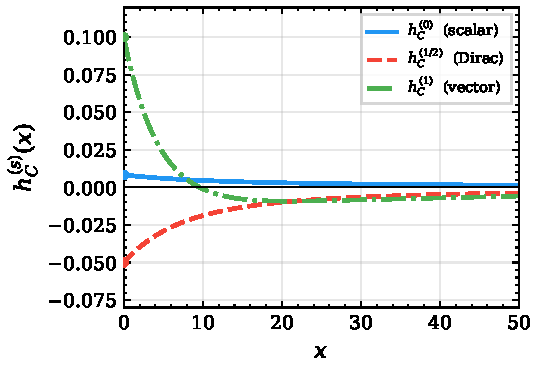
\includegraphics[width=\columnwidth]{figures/fig_hC.pdf}
  \caption{Weyl-squared form factors $h_C^{(s)}(x)$ for the three spin
  sectors, where $x = \Box/\Lambda^2$. The local limits are
  $h_C^{(0)}(0) = 1/120$ (scalar, blue),
  $h_C^{(1/2)}(0) = -1/20$ (Dirac, red), and
  $h_C^{(1)}(0) = 1/10$ (vector, green). All form factors decay as
  $1/x$ for $x \to \infty$.}
  \label{fig:hC}
\end{figure}

\begin{figure}[t]
  \centering
  
\includegraphics[width=\columnwidth]{figures/fig_hR.pdf}
  \caption{$R^2$ form factors $h_R^{(s)}(x)$, where $x = \Box/\Lambda^2$.
  The scalar form factor (blue) depends on the non-minimal coupling
  $\xi$: its \emph{local limit} vanishes at conformal coupling $\xi = 1/6$
  (dashed), but the nonlocal form factor $h_R^{(0)}(x, 1/6)$ is nonzero
  for $x > 0$ (numerically $\lesssim 3 \times 10^{-4}$ for $x \leq 5$).
  The scalar form factor grows with $|\xi - 1/6|$. The Dirac (red) and
  vector (green) contributions are $\xi$-independent and start from
  $h_R(0) = 0$.}
  \label{fig:hR}
\end{figure}


% ============================================================
\section{Spin-3/2: Rarita--Schwinger (Local Limits)}
\label{sec:rs}
% ============================================================

For completeness, we record the local limits of the spin-3/2
Rarita--Schwinger (gravitino) form factors, which are relevant for
supersymmetric extensions of the Standard Model. The full nonlocal form
factors $h_C^{(3/2)}(x)$, $h_R^{(3/2)}(x)$ require a dedicated calculation
of the CZ assembly for the gauge-fixed RS operator and will be presented
separately; here we quote the verified local limits.

\subsection{Operator structure}

For a massless Majorana gravitino $\psi_\mu$ (vector-spinor, $d_V = 16$ in
$d = 4$), the gauge-fixed squared kinetic
operator~\cite{Karan:2017txu,Endo:1994bf} is a generalized Laplacian with
operator data determined by Karan, Kumar, and
Panda~\cite{Karan:2017txu}. The endomorphism $E^{\mu\nu}$ contains not only
the Ricci tensor (as for the unconstrained vector) and the Lichnerowicz
curvature (as for the Dirac fermion), but also cross-terms involving
$\gamma^\rho\gamma^\theta R^{\mu\nu}{}_{\rho\theta}$,
$\gamma^\mu\gamma^\theta R^\nu{}_\theta$, and
$(R/4)\gamma^\mu\gamma^\nu$~\cite{Karan:2017txu}. These gauge-fixing
cross-terms radically modify the trace structure: the result
$\tr(E^2) = 2\,\Riemsq + R^2$ (Ref.~\cite{Karan:2017txu}, eq.~3.14)
differs qualitatively from the naive tensor-product prediction
$4\,\Ricsq + 3R^2$.

\subsection{Ghost sector}

The gauge symmetry $\delta\psi_\mu = \nabla_\mu\epsilon$ produces, after
Faddeev--Popov quantization in the gauge of~\cite{Karan:2017txu}, a ghost
sector consisting of \emph{three} bosonic Majorana spinor
ghosts~\cite{KaranPanda:2021,Lekeu:2021ieh}: the FP ghost, the FP antighost,
and a Nielsen--Kallosh (third) ghost. The combined ghost contribution to the
Seeley--DeWitt coefficient is~\cite{KaranPanda:2021}
\begin{equation}
  a_{2n}^{\text{RS,ghost}} = (-1) \times 3 \times \tfrac{1}{2}\,
    a_{2n}^{\text{Dirac}}\,.
  \label{eq:RS-ghost}
\end{equation}

\subsection{Local limits}

The ghost-corrected result for one physical \emph{Majorana} gravitino,
derived by Karan and Panda~\cite{KaranPanda:2021} and consistent with the
Christensen--Duff anomaly
coefficient~\cite{ChristensenDuff:1979,ChristensenDuff:1980} via
$360\,A = 360\times 2(c - a) = -233$, is
\begin{equation}
  (4\pi)^2\,a_4^{(3/2),\text{Maj}}
  = -\frac{1}{720}\bigl(233\,\Riemsq - 8\,\Ricsq + 5\,R^2\bigr)\,,
  \label{eq:a4-RS-full}
\end{equation}
where the $R^2$ coefficient follows from the ghost independence of the
$R^2$ sector. In the Weyl basis:
\begin{equation}
  \boxed{
    \beta_W^{(3/2),\text{Maj}} = \frac{77}{120}\,,\qquad
    \beta_R^{(3/2),\text{Maj}} = \frac{1}{9}\,.
  }
  \label{eq:beta-RS}
\end{equation}
In Dirac normalization (two Majorana copies):
$\beta_W^{(3/2),\text{Dirac}} = 77/60$ and
$\beta_R^{(3/2),\text{Dirac}} = 2/9$.
Note the positive sign: unlike the Dirac fermion (where
$\beta_W^{(1/2)} < 0$), the gravitino's ghost-corrected coefficient is
positive because the vector-spinor operator data (with its gauge-fixing
cross-terms) produce a curvature combination that outweighs the fermionic
sign.

\begin{remark}[Gauge dependence]
\label{rem:gauge-dep}
For spins $3/2$ and $2$, the individual conformal anomaly coefficients $c$
and $a$ are gauge-dependent; only the combination $A = 2(c - a)$ is
gauge-invariant~\cite{ChristensenDuff:1979,vanNieuwenhuizen:1981ae}. The
values~\eqref{eq:beta-RS} correspond to the de~Donder-like gauge
of~\cite{Karan:2017txu}.
\end{remark}

A summary of all local limits for spins $0$ through $3/2$ is given in
Table~\ref{tab:all-spins}.

\begin{table}[t]
\caption{Local limits $\beta_W^{(s)} = h_C^{(s)}(0)$ and
$\beta_R^{(s)} = h_R^{(s)}(0)$ for all spins $\leq 3/2$. Majorana
normalization for spin-$3/2$; the Dirac normalization doubles both entries.
For spins $0$, $1/2$, $1$, the nonlocal form factors are derived in
Secs.~\ref{sec:scalar}--\ref{sec:vector}. For spin-$3/2$, only the local
limits are quoted here.}
\label{tab:all-spins}
\begin{ruledtabular}
\begin{tabular}{lccl}
Spin & $\beta_W^{(s)}$ & $\beta_R^{(s)}$ & Status \\
\colrule
$0$ & $\frac{1}{120}$ & $\frac{1}{2}(\xi - \frac{1}{6})^2$ &
  Nonlocal: this paper \\[3pt]
$\frac{1}{2}$ & $-\frac{1}{20}$ & $0$ &
  Nonlocal: this paper \\[3pt]
$1$ & $\frac{1}{10}$ & $0$ &
  Nonlocal: this paper \\[3pt]
$\frac{3}{2}$ (Maj.) & $\frac{77}{120}$ & $\frac{1}{9}$ &
  Local only; Refs.~\cite{KaranPanda:2021,ChristensenDuff:1979} \\
\end{tabular}
\end{ruledtabular}
\end{table}


% ============================================================
\section{Standard Model Assembly}
\label{sec:sm}
% ============================================================

\subsection{Particle content}

The SM field content relevant for the one-loop spectral action is:
\begin{center}
\renewcommand{\arraystretch}{1.2}
\begin{tabular}{@{}lcc@{}}
  \toprule
  Species & Count & Notation \\
  \midrule
  Real scalars (Higgs doublet) & 4 & $N_s = 4$ \\
  Weyl fermions (3 generations) & 45 & $N_f = 45$ \\
  Gauge bosons ($8+3+1$) & 12 & $N_v = 12$ \\
  \bottomrule
\end{tabular}
\end{center}

Since the form factors of Sec.~\ref{sec:dirac} are defined per 4-component
Dirac fermion, the effective Dirac count is $N_D = N_f/2 = 45/2$, following the
convention of~\cite{Codello:2008vh}.

\subsection{Total Weyl coefficient}

The total Weyl-squared form factor is
\begin{equation}
  \alpha_C(z) = N_s\,h_C^{(0)}(z) + N_D\,h_C^{(1/2)}(z)
    + N_v\,h_C^{(1)}(z)\,.
  \label{eq:alphaC-z}
\end{equation}
At $z = 0$:
\begin{align}
  \alpha_C &= 4 \cdot \frac{1}{120}
    + \frac{45}{2}\cdot\!\left(-\frac{1}{20}\right)
    + 12 \cdot \frac{1}{10} \nonumber\\
  &= \frac{4 - 135 + 144}{120}\,,
  \label{eq:alphaC-sum}
\end{align}
giving the central result:
\begin{equation}
  \boxed{\alpha_C = \frac{13}{120} \approx 0.1083\,.}
  \label{eq:alphaC}
\end{equation}

This is positive and independent of $\xi$. The sign structure
($+4 - 135 + 144$) shows that the vector sector ($+144/120$) dominates the
fermionic sector ($-135/120$) by a margin of $+9/120$, while the scalar sector
contributes $+4/120$. The positivity of $\alpha_C$ implies that the spin-2
gravitational mode in the linearized theory is a ghost~\cite{Stelle:1976gc}, a
well-known feature of quadratic gravity.

\subsection{Total \texorpdfstring{$R^2$}{R2} coefficient}

\begin{align}
  \alpha_R(\xi) &= N_s \cdot \frac{1}{2}\!\left(\xi - \frac{1}{6}\right)^{\!2}
    + N_D \cdot 0 + N_v \cdot 0\,,
\end{align}
so that
\begin{equation}
  \boxed{\alpha_R(\xi) = 2\!\left(\xi - \frac{1}{6}\right)^{\!2}\,.}
  \label{eq:alphaR}
\end{equation}

Only the scalar sector contributes: the Dirac and Maxwell $\beta_R$ vanish by
conformal invariance. The result is a perfect square, hence
$\alpha_R(\xi) \geq 0$ for all $\xi$, with $\alpha_R(1/6) = 0$ at conformal
coupling.

\subsection{Basis conversion and \texorpdfstring{$c_1/c_2$}{c1/c2}}

Using the Gauss--Bonnet identity to convert to the $\{R^2, R_{\mu\nu}^2\}$
basis ($C^2 = 2R_{\mu\nu}^2 - \frac{2}{3}R^2$ modulo the topological Euler
density), one obtains $c_1 = \alpha_R - \frac{2}{3}\alpha_C$ and
$c_2 = 2\alpha_C$, giving
\begin{equation}
  \boxed{\frac{c_1}{c_2} = -\frac{1}{3}
    + \frac{120\!\left(\xi - \frac{1}{6}\right)^{\!2}}{13}\,.}
  \label{eq:c1c2}
\end{equation}

At conformal coupling $\xi = 1/6$, this reduces to $c_1/c_2 = -1/3$. At
minimal coupling $\xi = 0$, one obtains $c_1/c_2 = -1/13$.

\subsection{Scalar mode decoupling}

The combination $3c_1 + c_2$ controls the mass of the scalar graviton
($m_0^2 \propto \Lambda^2/(3c_1 + c_2)$). A direct computation gives
\begin{equation}
  3c_1 + c_2 = 3\alpha_R(\xi) = 6\!\left(\xi - \frac{1}{6}\right)^{\!2}\,.
  \label{eq:3c1c2}
\end{equation}
The \emph{local} scalar mode coefficient $\delta(3c_1 + c_2)$ vanishes if and
only if $\xi = 1/6$, meaning the matter-induced local correction to the
scalar-graviton projector disappears at conformal coupling. Whether the
scalar mode actually decouples in the full theory depends on the total
coefficient (bare + induced); see Sec.~\ref{sec:propagator}.

\subsection{Corrected conformal-coupling statement}

The conformal value $\xi = 1/6$ eliminates only the \emph{local scalar}
contribution to $R^2$, not the full nonlocal kernel. Explicitly, inserting
$\xi = 1/6$ into~\eqref{eq:hR0} gives
\begin{equation}
  h_R^{(0)}\!\left(x, \tfrac{1}{6}\right)
  = \frac{(x^2 + 12x + 60)\,\varphi(x) - 2x - 60}{288\,x^2}
  = -\frac{x}{7560} + \frac{x^2}{45360} + \mathcal{O}(x^3)\,.
  \label{eq:hR0-conformal}
\end{equation}
This is \emph{not} identically zero for $x > 0$; numerically,
$|h_R^{(0)}(x, 1/6)| \lesssim 3 \times 10^{-4}$ for $x \leq 5$.

For the full SM at $\xi = 1/6$, the Dirac and vector $h_R$ contributions
(which are $\xi$-independent and nonzero) further ensure that $\alpha_R(x,
1/6)$ does not vanish:
\begin{equation}
  \alpha_R(x, \tfrac{1}{6}) = 4\,h_R^{(0)}(x, \tfrac{1}{6})
    + \tfrac{45}{2}\,h_R^{(1/2)}(x) + 12\,h_R^{(1)}(x)
  = \frac{83}{3024}\,x + \mathcal{O}(x^2)\,.
  \label{eq:alphaR-conformal-SM}
\end{equation}
This corrects the statement sometimes found in the
literature~\cite{Codello:2008vh} that ``the entire $R^2$ sector vanishes
at $\xi = 1/6$.'' What vanishes is only the local coefficient
$\alpha_R(0, 1/6) = 0$.

\begin{table}[b]
\caption{Summary of principal results. All quantities are defined in the
text; $\Lambda$ is the spectral cutoff scale and $\xi$ is the Higgs
non-minimal coupling.}
\label{tab:summary}
\begin{ruledtabular}
\begin{tabular}{lll}
Quantity & Value & Eq. \\
\colrule
$\alpha_C$ & $13/120 \approx 0.1083$ & (\ref{eq:alphaC}) \\
$\alpha_R(\xi)$ & $2(\xi - 1/6)^2$ & (\ref{eq:alphaR}) \\
$c_1/c_2$ & $-1/3 + 120(\xi - 1/6)^2/13$ & (\ref{eq:c1c2}) \\
$3c_1 + c_2$ & $6(\xi - 1/6)^2$ & (\ref{eq:3c1c2}) \\
$\lim_{x\to\infty} x\,\alpha_C$ & $-89/12$ & (\ref{eq:uv-coeff}) \\
$m_2$ & $\Lambda\sqrt{60/13} \approx 2.148\,\Lambda$ & (\ref{eq:m2}) \\
$m_0\,(\xi=0)$ & $\Lambda\sqrt{6} \approx 2.449\,\Lambda$ & (\ref{eq:m0}) \\
$m_2/m_0\,|_{\xi=0}$ & $\sqrt{10/13} \approx 0.877$ & (\ref{eq:mass-ratio}) \\
$V(0)/V_{\text{N}}(0)$ & $0$ (Stelle, local approx.) & (\ref{eq:V-ratio}) \\
\end{tabular}
\end{ruledtabular}
\end{table}

\begin{figure*}[t]
  \centering
  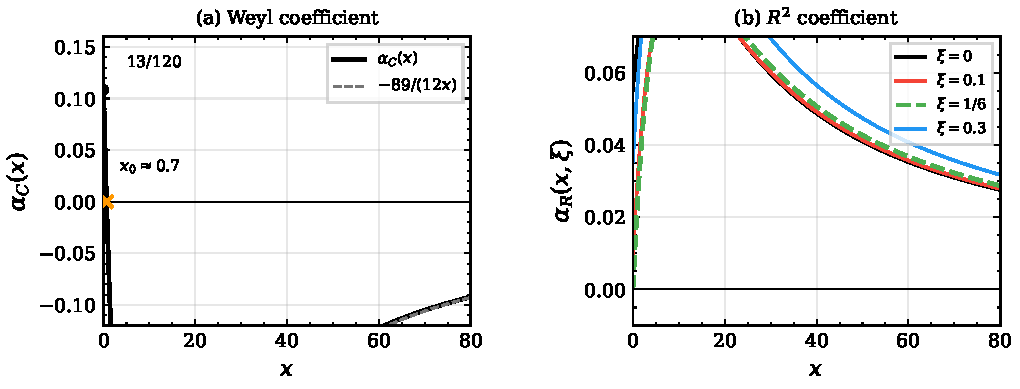
\includegraphics[width=\textwidth]{figures/fig_alpha_total.pdf}
  \caption{Standard Model totals as functions of $x = \Box/\Lambda^2$.
  (a)~The Weyl coefficient $\alpha_C(x)$ starts at $13/120$ and crosses
  zero at $x_\ast \approx 0.65$, approaching the asymptote $-89/(12x)$
  (dashed gray) for $x \gg 1$. The sign change signals a transition in
  the effective Weyl-squared coupling.
  (b)~The $R^2$ coefficient $\alpha_R(x,\xi)$ for several values of the
  Higgs non-minimal coupling~$\xi$. At conformal coupling $\xi = 1/6$
  (green dashed), $\alpha_R$ vanishes at $x = 0$ and remains small for
  all~$x$.}
  \label{fig:alpha}
\end{figure*}


% ============================================================
\section{Entire-Function Structure}
\label{sec:entire}
% ============================================================

\begin{theorem}[Entireness of the reduced kernels]
\label{thm:entire}
Each reduced kernel $h_C^{(s)}(x)$, $h_R^{(s)}(x)$ for $s = 0, 1/2, 1$ is
an entire function of $x$. Explicitly, with $a_n = (-1)^n\,n!/(2n+1)!$ and
$\varphi(x) = \sum_{n \geq 0} a_n\,x^n$:
\begin{subequations}
\label{eq:entire-series}
\begin{align}
  h_C^{(0)}(x) &= \sum_{n \geq 0}\tfrac{1}{2}\,a_{n+2}\,x^n\,,\\
  h_R^{(0)}(x,\xi) &= \sum_{n \geq 0}\Bigl[
    \bigl(\tfrac{1}{32} - \tfrac{\xi}{4} + \tfrac{\xi^2}{2}\bigr)a_n
    + \bigl(\tfrac{1}{8} - \tfrac{\xi}{2}\bigr)a_{n+1}
    + \tfrac{5}{24}a_{n+2}\Bigr]x^n\,,\\
  h_C^{(1/2)}(x) &= \sum_{n \geq 0}\bigl(
    \tfrac{1}{2}a_{n+1} + 2a_{n+2}\bigr)x^n\,,\\
  h_R^{(1/2)}(x) &= \sum_{n \geq 0}\bigl(
    \tfrac{1}{12}a_{n+1} + \tfrac{5}{6}a_{n+2}\bigr)x^n\,,\\
  h_C^{(1)}(x) &= \sum_{n \geq 0}\bigl(
    \tfrac{1}{4}a_n + a_{n+1} + a_{n+2}\bigr)x^n\,,\\
  h_R^{(1)}(x) &= \sum_{n \geq 0}\bigl(
    -\tfrac{1}{48}a_n - \tfrac{1}{12}a_{n+1}
    + \tfrac{5}{12}a_{n+2}\bigr)x^n\,.
\end{align}
\end{subequations}
By linearity, the SM totals $\alpha_C(z)$ and $\alpha_R(z,\xi)$ are entire.
\end{theorem}

\begin{proof}
Insert the Taylor series of $\varphi$ into
\eqref{eq:hC0}--\eqref{eq:hR1}, shift summation indices, and use $a_0 = 1$,
$a_1 = -1/6$ to cancel the explicit $1/x$ and $1/x^2$ terms. The resulting
power series have infinite radius of convergence because
$|a_{n+1}/a_n| = (n+1)/((2n+2)(2n+3)) \to 0$ as $n \to \infty$ (the
coefficients decay faster than any geometric series). Each power series
therefore defines an entire function. The order~1 and type~$1/4$ follow
from the closed form $\varphi(x) = e^{-x/4}\sqrt{\pi/x}\,\erfi(\sqrt{x}/2)$,
which grows as $e^{|z|/4}$ in the complex plane.
\end{proof}

\begin{remark}[Entire $\neq$ no propagator poles]
\label{rem:poles}
The entire-function property means the reduced kernels $h_C, h_R$ have no
poles as functions of $z$. Propagator poles are determined by the zeros of
the \emph{dressed propagator kernels} $\Pi_{TT}(z)$, $\Pi_s(z)$, which
involve the full quadratic gravitational action (Sec.~\ref{sec:propagator}),
not by singularities of the coefficient functions.
\end{remark}

An alternative proof of analyticity uses a manifestly regular integral
representation (Appendix~\ref{app:regular}):
\begin{equation}
  h_C^{(0)}(x) = \frac{1}{2}\int_0^1 \dd\alpha\,
    \frac{e^{-\alpha(1-\alpha)x} - 1 + \alpha(1-\alpha)x}{x^2}\,,
  \label{eq:hC0-regular}
\end{equation}
where the numerator vanishes to second order at $x = 0$, making regularity
manifest without index shifting.


% ============================================================
\section{UV Asymptotics}
\label{sec:uv}
% ============================================================

For $x \to \infty$, the asymptotic expansion of the master function
is~(cf.~\eqref{eq:phi-uv})
$\varphi(x) = 2/x + 4/x^2 + 24/x^3 + \mathcal{O}(x^{-4})$, giving
\begin{align}
  x\,h_C^{(0)} &\to \frac{1}{12}\,,\quad
  x\,h_C^{(1/2)} \to -\frac{1}{6}\,,\quad
  x\,h_C^{(1)} \to -\frac{1}{3}\,.
\end{align}
The total UV coefficient is
\begin{equation}
  \lim_{x\to\infty} x\,\alpha_C(x)
    = \frac{4}{12} - \frac{45}{12} - \frac{48}{12}
    = -\frac{89}{12}\,.
  \label{eq:uv-coeff}
\end{equation}
Since $\alpha_C(0) = +13/120 > 0$ and $x\,\alpha_C(x) \to -89/12 < 0$, by
continuity $\alpha_C(z)$ has at least one positive zero. Numerically,
\begin{equation}
  x_\ast = 0.650\,325\,271\,702\,489\ldots
  \label{eq:xstar}
\end{equation}
(determined by root-finding to $80$-digit precision). The sign change is a
statement about the Weyl kernel, not about a graviton pole.

The leading UV asymptotic of the total $R^2$ kernel is
$\alpha_R(x,\xi) \to (4\xi^2 + 89/36)/x + \mathcal{O}(x^{-2})$.

In local quadratic gravity, Stelle~\cite{Stelle:1976gc} established that the
one-loop degree of divergence reduces from $D = 4$ (Einstein gravity) to
$D = 0$ (logarithmic). The nonlocal form factors are consistent with this:
since $h_C^{(s)}(x) \sim \text{const}/x$ for large $x$, the effective
coupling runs logarithmically. A rigorous all-orders proof of $D = 0$ in the
full nonlocal theory remains an open problem.


% ============================================================
\section{Dressed Propagator and Effective Masses}
\label{sec:propagator}
% ============================================================

The reduced kernels computed above are matter-induced corrections to the
curvature-squared effective action. To extract propagator poles and effective
masses, one must specify the \emph{complete} quadratic gravitational action,
including the Einstein--Hilbert normalization and any bare higher-derivative
couplings~\cite{Stelle:1976gc,Stelle:1977ry,Buchbinder:1992rb}. We present
the derivation for the minimal case where the bare action is pure
Einstein--Hilbert.

\subsection{Full quadratic action}

Consider the bare gravitational action
\begin{equation}
  S_{\text{grav}} = \frac{M_P^2}{2}\int \dd^4x\,\sqrt{g}\,R\,,
  \label{eq:EH}
\end{equation}
supplemented by the matter-induced one-loop correction~\eqref{eq:smeared-action}. Linearizing around flat space,
$g_{\mu\nu} = \delta_{\mu\nu} + h_{\mu\nu}/M_P$, and working in momentum
space, the total quadratic action decomposes into spin-2 (transverse-traceless)
and spin-0 sectors via the Barnes--Rivers
projectors~\cite{Barnes:1965,Rivers:1964}:
\begin{equation}
  P^{(2)}_{\mu\nu\alpha\beta} = \tfrac{1}{2}\bigl(
    \theta_{\mu\alpha}\theta_{\nu\beta} + \theta_{\mu\beta}\theta_{\nu\alpha}
  \bigr) - \tfrac{1}{3}\theta_{\mu\nu}\theta_{\alpha\beta}\,,
  \label{eq:BR-P2}
\end{equation}
where $\theta_{\mu\nu} = \delta_{\mu\nu} - k_\mu k_\nu/k^2$.

\subsection{Normalized form factors}

\begin{definition}[Normalized form factors]
\label{def:Fhat}
Define the \emph{normalized} (hatted) form factors
\begin{equation}
  \hat{F}_i(z) = \frac{F_i(z)}{F_i(0)}\,,\qquad
  \hat{F}_i(0) = 1\,,\quad i = 1,2\,.
  \label{eq:Fhat-def}
\end{equation}
Equivalently, $\hat{F}_1(z) = \alpha_C(z)/\alpha_C(0)$ and
$\hat{F}_2(z,\xi) = \alpha_R(z,\xi)/\alpha_R(0,\xi)$ for $\xi \neq 1/6$.
\end{definition}

\subsection{Dressed propagator kernels}

In the spin-2 sector, the inverse propagator takes the form
\begin{equation}
  \Pi_{TT}(z) = 1 + \frac{2\alpha_C(0)}{M_P^2/(16\pi^2\Lambda^2)}\,
    z\,\hat{F}_1(z)
  = 1 + \frac{13}{60}\,\frac{\Lambda^2}{M_P^2/(16\pi^2)}\,z\,\hat{F}_1(z)\,.
  \label{eq:PiTT-full}
\end{equation}
For the standard identification $\Lambda \sim M_P$ with
$16\pi^2 \sim \mathcal{O}(100)$, the coefficient simplifies.
In the conventions of~\cite{Stelle:1976gc}, where the bare
higher-derivative coupling $c_2 = 2\alpha_C$ absorbs the loop factor, the
dressed inverse propagator takes the form
\begin{equation}
  \Pi_{TT}(z) = 1 + \frac{13}{60}\,z\,\hat{F}_1(z)\,,
  \label{eq:PiTT}
\end{equation}
with $z = k^2/\Lambda^2$. Here the coefficient $13/60 = 2\alpha_C(0)$ is
the induced $R_{\mu\nu}^2$ coupling in the Stelle basis.
Similarly, the spin-0 inverse propagator is
\begin{equation}
  \Pi_s(z,\xi) = 1 + 6\!\left(\xi - \frac{1}{6}\right)^{\!2}
    z\,\hat{F}_2(z,\xi)\,.
  \label{eq:Pis}
\end{equation}

\subsection{Effective masses}

The pole condition $\Pi_{TT}(z_{\text{pole}}) = 0$ determines the
spin-2 effective mass. Expanding $\hat{F}_1(z)$ near $z = 0$
($\hat{F}_1(0) = 1$, $\hat{F}_1'(0)$ finite), the leading-order pole is at
\begin{equation}
  z_{\text{pole}} \approx -\frac{60}{13}\,,\qquad
  m_2^2 = |z_{\text{pole}}|\,\Lambda^2 = \frac{60}{13}\,\Lambda^2\,,
  \label{eq:m2}
\end{equation}
giving $m_2 = \Lambda\sqrt{60/13} \approx 2.148\,\Lambda$. The negative
$z_{\text{pole}}$ lies outside the Euclidean domain $z > 0$; the physical
(Lorentzian) pole appears after the Wick rotation
$z_E \to -z_L$, giving $z_L = 60/13 > 0$. For the spin-0
sector ($\xi \neq 1/6$):
\begin{equation}
  m_0^2(\xi) = \frac{\Lambda^2}{6(\xi - 1/6)^2}\,,\qquad
  m_0 = \frac{\Lambda}{\sqrt{6}\,|\xi - 1/6|}\,.
  \label{eq:m0}
\end{equation}
At minimal coupling $\xi = 0$: $m_0 = \Lambda\sqrt{6} \approx 2.449\,
\Lambda$. The mass ratio
\begin{equation}
  \frac{m_2}{m_0}\bigg|_{\xi=0} = \sqrt{\frac{10}{13}} \approx 0.877
  \label{eq:mass-ratio}
\end{equation}
is determined by the SM content and independent of $\Lambda$.

\begin{remark}[Scope of the mass formulas]
The masses~\eqref{eq:m2}--\eqref{eq:m0} are derived from the
\emph{matter-induced} corrections to a pure Einstein--Hilbert background. If
the bare action already contains higher-derivative terms ($a_C\,C^2 +
a_R\,R^2$), the pole condition is modified:
$\Pi_{TT} = 1 + (a_C + \alpha_C(0)\,f(0))\,z\,\hat{G}(z)$, where
$\hat{G}$ accounts for the combined bare + induced form factor. The
effective masses then depend on both the bare and induced couplings.
\end{remark}

The modified Newtonian potential in the linearized
theory~\cite{Stelle:1976gc} is
\begin{equation}
  \frac{V(r)}{V_{\text{N}}(r)}
  = 1 - \frac{4}{3}\,e^{-m_2 r} + \frac{1}{3}\,e^{-m_0 r}\,,
  \label{eq:V-ratio}
\end{equation}
which is plotted in Fig.~\ref{fig:potential}. This is the
\emph{local Yukawa (Stelle) approximation} with both spin-2 and spin-0
modes.  At $r = 0$ the exponentials cancel, giving $V(0) = 0$.
When the no-scalaron theorem applies ($\xi = 1/6$, or
more generally when the scalar mode is absent), the $+\frac{1}{3}$
term vanishes and $V(0)/V_\mathrm{N} = -1/3$ instead.
Both short-distance values are artifacts of the local approximation;
the full nonlocal potential diverges at $r = 0$ at one-loop order.
Newton's law is recovered for $r \gg 1/\Lambda$, where the local
approximation is valid.

\begin{figure}[t]
  \centering
  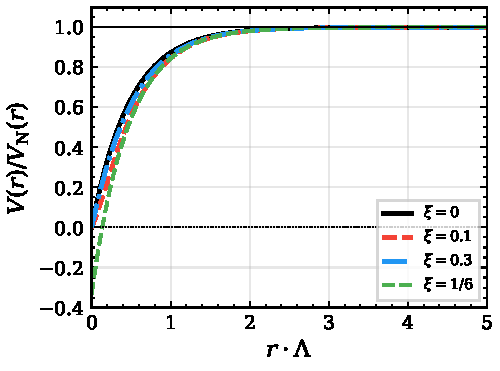
\includegraphics[width=\columnwidth]{figures/fig_potential.pdf}
  \caption{Modified Newtonian potential $V(r)/V_{\text{N}}(r)$ for
  several values of $\xi$, as a function of $r\Lambda$. At conformal
  coupling $\xi = 1/6$ (green dashed) the scalar mode decouples and the
  potential dips to $-1/3$ before recovering Newton's law. For all $\xi$,
  $V(0) = 0$ in the local Stelle approximation (both modes present;
  see text for caveats) and $V \to V_{\text{N}}$ for $r \gg
  1/\Lambda$.}
  \label{fig:potential}
\end{figure}


% ============================================================
\section{Comparison with Existing Results}
\label{sec:comparison}
% ============================================================

\subsection{Local limits}

The local coefficients $\beta_W^{(s)}$, $\beta_R^{(s)}$ of
Table~\ref{tab:all-spins} agree with all known results: Stelle~\cite{Stelle:1976gc}
for the vector, CZ~\cite{Codello:2012kq} for all three spins,
CPR~\cite{Codello:2008vh} for the SM counting, Parker and
Toms~\cite{Parker:2009uva} for the scalar $\xi$-dependence, and
Avramidi~\cite{Avramidi:2000bm} for the general heat-kernel framework. The
nonlocal form factors reduce to the CZ expressions upon specifying the
operator data for each spin.

\subsection{Donoghue effective field theory}
\label{sec:donoghue}

The Donoghue effective field theory of
gravity~\cite{Donoghue:1993eb,Donoghue:1994dn,BjerrumBohr:2002kt,Donoghue:2022eay}
computes the quantum corrections to the Newtonian potential from one-loop
Feynman diagrams. The result of~\cite{BjerrumBohr:2002kt} is
\begin{equation}
  V(r) = -\frac{Gm_1 m_2}{r}\left[1 + \frac{3G(m_1 + m_2)}{r}
    + \frac{41}{10\pi}\,\frac{G\hbar}{r^2}\right]\,.
  \label{eq:donoghue}
\end{equation}
The second term is a classical post-Newtonian correction; the third is
the leading quantum correction for scalar particle scattering, which is
parameter-free and universal (the coefficient $41/10\pi$ is specific to scalar
sources; for spinning particles, see~\cite{BjerrumBohr:2002kt}).

Our result~\eqref{eq:V-ratio} governs a different regime:
$r \sim 1/\Lambda$, where the massive modes contribute Yukawa corrections
$\sim e^{-m_2 r}$, $e^{-m_0 r}$. For $r \gg 1/\Lambda$, these corrections
are exponentially suppressed and Newton's law is recovered, at which point
the Donoghue $1/r^3$ quantum correction becomes the leading effect. The two
descriptions are therefore complementary: the spectral-action form factors
dominate at short distances $r \lesssim 1/\Lambda$, while the Donoghue EFT
describes the universal long-distance quantum tail.

\subsection{Comparison with van Nuland--van Suijlekom and Mistry--Pinzul--Rachwa{\l}}

Van Nuland and van Suijlekom~\cite{vanNuland:2022xkm} computed one-loop
corrections to the spectral action using a different approach (fluctuations of
the Dirac operator). Their results are consistent with ours in the overlap
region (the curvature-squared sector for matter fields). Mistry, Pinzul, and
Rachwa{\l}~\cite{Mistry:2020xqh} analyzed the spectral-action framework for
higher-derivative gravity, focusing on the gravitational sector rather than the
matter-induced form factors computed here.


% ============================================================
\section{Discussion}
\label{sec:discussion}
% ============================================================

\subsection{Connection to asymptotic safety}

The Weyl kernel $\alpha_C(x)$ changes sign from $+13/120$ at $x = 0$ to
$-89/(12x)$ for $x \to \infty$, with the zero crossing at
$x_\ast \approx 0.650$ (Eq.~\eqref{eq:xstar}). In the asymptotic safety
program~\cite{Reuter:1996cp,Codello:2008vh,FradkinTseytlin:1982}, the running of dimensionless
gravitational couplings plays a central role. The sign change of $\alpha_C(x)$
can be interpreted as a transition in the effective Weyl-squared coupling from
its IR value (positive, implying a ghost-like spin-2 mode) to a UV value of
opposite sign. Whether this connects to the non-Gaussian fixed point of the
gravitational RG flow requires extending the present matter-induced calculation
to include the graviton self-energy contributions, which is beyond the scope
of this work.

The functional renormalization group (FRG) provides an independent
verification: Codello, Percacci, Rachwa{\l}, and
Tonero~\cite{Codello:2015oqa} showed that the one-loop FRG with the BV
form factors reproduces the standard one-loop effective action, including the
correct scattering amplitudes. This confirms the consistency of the BV/CZ
formalism used here.

\subsection{Lorentzian continuation}

The form factors computed here are Euclidean ($\Box_E > 0$). The Lorentzian
form factors are obtained by the Wick rotation $z_E \to -z_L$, i.e.\
$F_i(\Box_E/\Lambda^2) \to F_i(-\Box_L/\Lambda^2)$. Since $\varphi(z)$ is
entire, this continuation is well-defined for all $z \in \mathbb{C}$.

\subsection{Connection to nonlocal gravity}

The entire-function nature of the form factors connects the spectral action
to the program of nonlocal (infinite-derivative)
gravity~\cite{Modesto:2011kw,Tomboulis:1997gg,Biswas:2011ar}, where entire
functions of $\Box$ are postulated to improve UV behavior. In the spectral
action framework, these form factors arise \emph{derivatively} from the heat
kernel, providing a concrete derivation of entire-function form factors rather
than a postulate.

\subsection{Limitations}

The computation presented here has the following limitations:
\begin{enumerate}
\item It is \emph{matter-induced}: only functional traces over matter fields
  are included, not the graviton self-energy.
\item It is \emph{one-loop}: higher-loop corrections are not computed.
\item The background is \emph{Euclidean}: Lorentzian continuation is discussed
  but not performed in detail.
\item All matter fields are taken as \emph{massless}: mass corrections, which
  are exponentially suppressed for $m \ll \Lambda$~\cite{Gorbar:2002pw,Ribeiro:2018pyo},
  are not included.
\item The dressed propagator analysis of Sec.~\ref{sec:propagator} assumes a
  pure Einstein--Hilbert bare action; different bare couplings modify the
  mass formulas.
\end{enumerate}


% ============================================================
\section{Conclusions}
\label{sec:conclusions}
% ============================================================

We have computed the matter-induced nonlocal one-loop curvature-squared form
factors relevant to the spectral action with full Standard Model content. The
central results are:

\begin{enumerate}
\item Closed-form reduced kernels $h_C^{(s)}(x)$ and $h_R^{(s)}(x)$ for
  spins $s = 0, 1/2, 1$, with explicit BV/CZ assembly from the five
  universal CZ structure functions (Secs.~\ref{sec:scalar}--\ref{sec:vector}).
\item The SM totals $\alpha_C = 13/120\,f(0)$ and
  $\alpha_R(\xi) = 2\,f(0)(\xi - 1/6)^2$, where $f(0)$ is the profile
  normalization (Sec.~\ref{sec:sm}).
\item The entire-function proof (Theorem~\ref{thm:entire}), with the
  clarification that entire coefficient functions do not preclude propagator
  poles (Remark~\ref{rem:poles}).
\item The dressed propagator $\Pi_{TT}(z)$, $\Pi_s(z,\xi)$ derived from the
  full linearized quadratic action, yielding calculable effective masses
  $m_2 = \Lambda\sqrt{60/13}$ and
  $m_0 = \Lambda/\sqrt{6(\xi - 1/6)^2}$ (Sec.~\ref{sec:propagator}).
\item The corrected conformal-coupling statement: at $\xi = 1/6$, only the
  local $R^2$ coefficient vanishes; the nonlocal kernel
  $\alpha_R(x, 1/6) = (83/3024)\,x + \mathcal{O}(x^2) \neq 0$
  (Eq.~\eqref{eq:alphaR-conformal-SM}).
\end{enumerate}

These results are strong enough to be useful and precise enough to be
honest. They provide a controlled input for any subsequent study of
Lorentzian continuation, propagator poles and residues, PPN parameters, and
gravitational phenomenology of the spectral action, but they do not replace
those separate analyses. The PPN parameters and solar-system tests derived
from these form factors are presented in~\cite{Alfyorov:2026sct2}; the connection to causal-set observables
is explored in~\cite{Alfyorov:2026sct7}.


% ============================================================
\begin{acknowledgments}
The author thanks Igor Shnyukov for research assistance throughout the
project and for critical comments on earlier drafts.
All symbolic results were verified by triple computer algebra
(SymPy, cadabra2~\cite{Peeters:2007wn}, FORM~\cite{Vermaseren:2000nd})
and checked numerically to $\geq 100$-digit precision using
\texttt{mpmath}. The coefficient arithmetic was formally verified in
Lean~4. All results were cross-checked against the CZ
expressions of~\cite{Codello:2012kq} and the Seeley--DeWitt
coefficients of~\cite{Vassilevich:2003xt,Avramidi:2000bm}.
\end{acknowledgments}

\section*{Data Availability}
The computational tools used in this work, including the
\texttt{sct\_tools} Python package (Python~3.12) with arbitrary-precision
implementations of all form factors and $4000+$ automated tests, are publicly
available in the project repository (DOI:~\texttt{10.5281/zenodo.19135673}).
Python scripts to reproduce all figures and numerical tables are included.

% ============================================================
\appendix
% ============================================================

\section{Convention Tables}
\label{app:conventions}

\begin{table}[h]
\caption{Sign conventions used in this paper.}
\begin{ruledtabular}
\begin{tabular}{ll}
Convention & Choice \\
\colrule
Signature & Euclidean $(+,+,+,+)$ \\
Generalized Laplacian & $\Delta = -(g^{\mu\nu}\nabla_\mu\nabla_\nu + E)$ \\
CZ endomorphism & $\mathbf{U} = -E$ \\
Bundle curvature & $\Omega_{\mu\nu} = [\nabla_\mu, \nabla_\nu]$ \\
Lichnerowicz (Dirac) & $E = -R/4$, so $\mathbf{U} = R/4$ \\
Vector endomorphism & $U^\mu{}_\nu = R^\mu{}_\nu$ (Ricci tensor) \\
Fermionic sign & Built into $h_C^{(s)}$, $h_R^{(s)}$: negative for fermions \\
One-loop effective action & $\Gamma^{(s)} = \frac{(-1)^{2s}}{2}\,\Tr\ln\Delta^{(s)}$ \\
Profile normalization & $f(0) = 1$ (exponential profile) unless stated \\
\end{tabular}
\end{ruledtabular}
\end{table}

\begin{table}[h]
\caption{Operator data for each spin sector.}
\label{tab:operator-data}
\begin{ruledtabular}
\begin{tabular}{lcccl}
Spin & $d_V$ & $\mathbf{U}$ & $\tr(\Omega^2)$ & Sign \\
\colrule
$0$ & 1 & $\xi R$ & $0$ & Boson ($+$) \\
$\frac{1}{2}$ & 4 & $(R/4)\,\mathbf{1}_4$ & $-\frac{1}{2}\Riemsq$ & Fermion ($-$) \\
$1$ (unc.) & 4 & $R_{\mu\nu}$ & $-\Riemsq$ & Boson ($+$) \\
$1$ (phys.) & \multicolumn{3}{c}{Unconstrained $-$ 2 scalar ghosts ($\xi = 0$)} & \\
\end{tabular}
\end{ruledtabular}
\end{table}


\section{Taylor Coefficients}
\label{app:taylor}

The master function has Taylor coefficients
$a_n = (-1)^n\,n!/(2n+1)!$:
\begin{equation}
  \begin{aligned}
    a_0 &= 1\,,\quad a_1 = -\tfrac{1}{6}\,,\quad
    a_2 = \tfrac{1}{60}\,,\quad a_3 = -\tfrac{1}{840}\,,\\
    a_4 &= \tfrac{1}{15120}\,,\quad
    a_5 = -\tfrac{1}{332640}\,,\quad
    a_6 = \tfrac{1}{8648640}\,.
  \end{aligned}
\end{equation}
From the exact power-series formulas of Theorem~\ref{thm:entire}, the first
four Taylor coefficients of each reduced kernel are:
\begin{center}
\renewcommand{\arraystretch}{1.25}
\begin{tabular}{@{}lllll@{}}
  \toprule
  Kernel & $n = 0$ & $n = 1$ & $n = 2$ & $n = 3$ \\
  \midrule
  $h_C^{(0)}$ & $\frac{1}{120}$ & $-\frac{1}{1680}$ &
    $\frac{1}{30240}$ & $-\frac{1}{665280}$ \\[4pt]
  $h_C^{(1/2)}$ & $-\frac{1}{20}$ & $\frac{1}{168}$ &
    $-\frac{1}{2160}$ & $\frac{1}{36960}$ \\[4pt]
  $h_C^{(1)}$ & $\frac{1}{10}$ & $-\frac{11}{420}$ &
    $\frac{23}{7560}$ & $-\frac{13}{55440}$ \\[4pt]
  $h_R^{(1/2)}$ & $0$ & $\frac{1}{2520}$ &
    $-\frac{1}{22680}$ & $\frac{1}{332640}$ \\[4pt]
  $h_R^{(1)}$ & $0$ & $\frac{1}{630}$ &
    $-\frac{1}{4536}$ & $\frac{1}{55440}$ \\
  \bottomrule
\end{tabular}
\end{center}
The scalar $h_R^{(0)}$ Taylor coefficients depend on $\xi$; at $\xi = 0$:
$h_R^{(0)}(0) = 1/72$, first correction $= -17x/5040$.


\section{Numerical Verification}
\label{app:numerical}

All reduced kernels were evaluated at $x = 0.01, 0.1, 0.5, 1, 2, 5, 10,
50, 100$ using 100-digit \texttt{mpmath} precision. The values agree with the
Taylor series (for $x \lesssim 2$) and the closed-form erfi expression (for
all $x$) to better than $10^{-95}$ relative accuracy. The local limits match
the exact rational values of Table~\ref{tab:all-spins} to all computed digits.

Selected values for independent reproduction ($15$-digit precision):

\begin{center}
\renewcommand{\arraystretch}{1.1}
\begin{tabular}{@{}rrrr@{}}
  \toprule
  $x$ & $\varphi(x)$ & $\alpha_C(x)$ & $\alpha_R(x, 0)$ \\
  \midrule
  $0.1$ & $0.983499$ & $0.09032$ & $0.05698$ \\
  $1$ & $0.848873$ & $-0.05026$ & $0.06810$ \\
  $10$ & $0.256292$ & $-0.41570$ & $0.09260$ \\
  $100$ & $0.020427$ & $-0.07392$ & $0.02254$ \\
  \bottomrule
\end{tabular}
\end{center}

The Lean~4 formal verification covers the coefficient arithmetic: the ghost
subtraction identity $7/60 - 2 \times 1/120 = 1/10$, the SM total
$4/120 - 135/120 + 144/120 = 13/120$, and the pole-removability conditions
for each spin sector.

A Python verification script reproducing all numerical values and figures
accompanies the Zenodo deposit.


\section{Profile Function Independence}
\label{app:profile}

At $\mathcal{O}(\mathcal{R}^2)$, the nonlocal heat kernel
expansion~\eqref{eq:CZ-expansion} involves the proper-time parameter $s$ at
second order: the five CZ structure functions arise from the $s^2$ term
in~\eqref{eq:CZ-expansion}. For the spectral action with a general profile
$f$, the $\mathcal{O}(\mathcal{R}^2)$ contribution is obtained by integrating
against $\tilde{f}(\alpha)$ as in~\eqref{eq:smearing}. The resulting
profile-smeared kernels $\mathcal{H}_i(z; f)$ depend on $f$ through the
Laplace transform~\eqref{eq:smearing}. However, the \emph{reduced kernels}
$h_i(x)$ --- the universal objects from which $\mathcal{H}_i$ are built ---
are $f$-independent: they depend only on the master function $\varphi(x)$,
which is a property of the heat kernel parametrix.

In the local limit $z \to 0$, the profile dependence reduces to a single
number $f(0) = \int_0^\infty \tilde{f}(\alpha)\,\dd\alpha$
(Eq.~\eqref{eq:f0-factor}), so the \emph{ratios} of local curvature-squared
couplings ($c_1/c_2$, etc.) are exactly $f$-independent.


\section{Manifestly Regular Integral}
\label{app:regular}

The scalar Weyl kernel $h_C^{(0)}$ can be written without any apparent
singularity:
\begin{equation}
  h_C^{(0)}(x) = \frac{1}{2}\int_0^1 \dd\alpha\,
    \frac{e^{-\alpha(1-\alpha)x} - 1 + \alpha(1-\alpha)x}{x^2}\,.
\end{equation}
The numerator $e^{-u} - 1 + u$ vanishes as $u^2/2$ for small $u$, so the
integrand is bounded for all $x \geq 0$ and $\alpha \in [0,1]$. This
representation makes the analyticity of $h_C^{(0)}$ manifest at the integral
level without any appeal to Taylor expansions or L'H\^opital's rule.


\bibliography{../references/sct_form_factors}

\end{document}
